\chapter{Design del sistema}

\section{Design Goals}
Il design di un sistema software deve essere svolto a valle di un'attenta 
analisi degli obiettivi di design, tradeoffs nell'ambito delle qualitá del 
software che rendano il software il piú adatto possibile per le sue ragioni 
di essere.

Il design del sistema deve essere costruito a partire dai requisiti non funzionali
descritti nel capitolo precedente.

\section{Design di alto livello}
Il sistema è suddiviso in due macro-componenti distribuite, comunicanti tramite 
rete:
\begin{list}{$\cdot$}{}
    \item Front-end. Il software che fornisce l'interfaccia con l'utente. Il front-end 
    interroga il back-end e restituisce le risposte che riceve da quest'ultimo.
    \item Back-end, detentore del Core, in cui viene gestita la logica di gestione delle 
    richieste e di manipolazione dei dati. Nel flusso di esecuzione, il Core è preceduto 
    da un Load Balancer, un middleware che gestisce il flusso di richieste per garantire 
    bilanciamento del carico tra le istanze del backend. I dati strutturati (entitá) sono 
    salvati su un DBMS, mentre i dati non strutturati (blob, immagini) sono salvati su un 
    Object Storage.
\end{list}

L'inserimento di una CDN (Content Delivery Network) é stato valutato e rimandato al 
futuro in quanto la geo-distribuzione non è, per adesso, obiettivo del sistema.

Sia front-end che back-end verranno descritti piú a fondo nelle sezioni successive.

\begin{figure}[h]
    \centering
    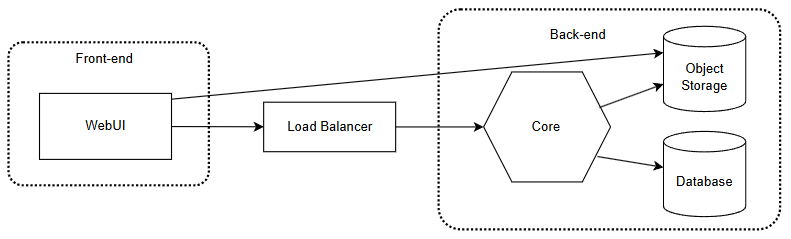
\includegraphics[width=\textwidth]{assets/diagrams/high-level-arch.png}
    \caption{L'architettura di alto livello}
    \label{fig:Architettura di alto livello}
\end{figure}

\begin{figure}[h]
    \centering
    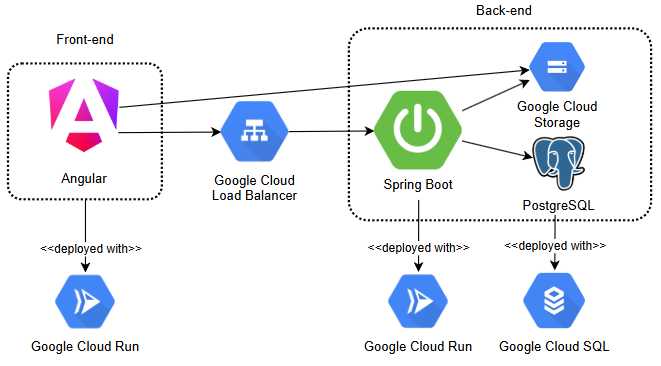
\includegraphics[width=\textwidth]{assets/diagrams/high-level-arch-tecnologies.png}
    \caption{L'architettura di alto livello, con tecnologie}
    \label{fig:Architettura di alto livello, con tecnologie}
\end{figure}

L'infrastruttura scelta per il deployment é Google Cloud, che garantisce availability 
di 99.95\% per i servizi di Run, SQL, Storage, per cui garantisce anche una durability 
ad undici 9.

Angular é stato scelto per implementare il front-end con una SPA (Single Page 
Application). La scelta di un'interfaccia web è figlia dell'obiettivo di alta 
adaptability.

Spring Boot é stato scelto per l'implementazione del core del sistema grazie al ridotto 
time-to-market che esso garantisce e alla sua affidabilitá dovuta al suo massiccio 
utilizzo nell'industria moderna. Spring Boot permette una facile integrazione di un 
potente ORM (Object Relational Mapping) come JPA (Java Persistence API).

PostgreSQL è stato scelto come DBMS per la sua efficienza e per il suo supporto nativo 
ai dati geografici (estensione PostGIS).

La scelta di un unico Cloud Provider permette una riduzione notevole della latenza nelle 
comunicazioni tra i componenti del sistema.

\section{Design del back-end}
\subsection{L'architettura esagonale}
La scelta di un framework opinionated come Spring Boot impone un’architettura ben precisa: 
architettura esagonale, anche detta port-and-adapters, formalizzata da A. Cockburn.

L’obiettivo di questa architettura é rendere il cosiddetto core facilmente testabile, 
manutenibile e molto agile di fronte a cambiamenti ed estensioni, permettendo di non 
stravolgere la codebase.

Per ottenere ciò, l’architettura esagonale definisce un confine netto tra il core e 
le estensioni, chiamate porte, che definiscono un contratto tra il core ed il componente 
esterno che fornisce l’estensione. Tale componente esterno é chiamato adapter.
Bisogna fare un distinguo tra porte in entrata e porte in uscita:
\begin{list}{$\cdot$}{}
    \item porte in entrata, spesso chiamate Service come nel caso di Spring, sono spesso 
    mappate a use case e definiscono possibili microservizi.
    \item porte in uscita sono interfacce che definiscono come il core puó utilizzare 
    un componente esterno.
\end{list}

Tale distinguo si riflette sugli adapter:
\begin{list}{$\cdot$}{}
    \item adapter in entrata, spesso chiamati Controller come nel caso di Spring, 
    usano le porte in entrata.
    \item adapter in uscita implementano le porte in uscita.
\end{list}

Sia le porte che gli adapter per la persistenza dei dati sono spesso chiamate Repository, 
come nel caso di Spring.

L’architettura esagonale: 
\begin{list}{$\cdot$}{}
    \item permette un testing efficace del core grazie alla dependency injection 
    alla base: il mocking delle dipendenze è molto semplificato.
    \item facilita l’aggiunta di nuove feature: si definisce una porta e la si 
    adatta con una tecnologia specifica.
    \item permette una migrazione naturale ad architetture piú modulari dal punto 
    di vista del deployment, come modular monolith e microservizi.
\end{list}

\subsection{Design}
%Insert the design diagram
%Insert the class diagram
%Insert the model class diagram

\section{Design del front-end}